\subsection{(111)-Goldschicht}
Die Rauheit der Goldschicht sollte mit dem RTM bestimmt werden. Dazu wurde die Oberfl�che der Goldschicht mit dem RTM im CC-Mode abgerastert.
Wegen der Kornstruktur wurden f�r die Bestimmung der Fl�chenrauheit zwei Messungen vorgenommen, sodass Korngrenzen nur in der ersten Messung in die Berechnung der Rauheit eingingen. Die (111)-Goldschicht musste aufgrund von Kratzern auf der Oberfl�che mehrfach gedreht werden. W�hrend der Justierung ist die Pt-Ir-Spitze des RTM mit der Oberfl�che der Goldschicht kollidiert, sodass eine zweite Pt-Ir-Spitze angefertigt werden musste. Diese konnte ebenfalls nach wenigen Versuchen aus bereits benutzten Pt-Ir-Spitzen angefertigt werden. Zu erste wird eine Aufnahme mit maximalem Scanbereich gemacht, dabei wird die tip-Voltage von 50mV auf 500mV erh�ht, um ein sch�rferes Bild zu erhalten. In Abbildung \ref{fig:gold_maximal_scan} ist die Aufnahme mit maximalem Scanbereich zu sehen.

\begin{figure}[H]
	\centering
  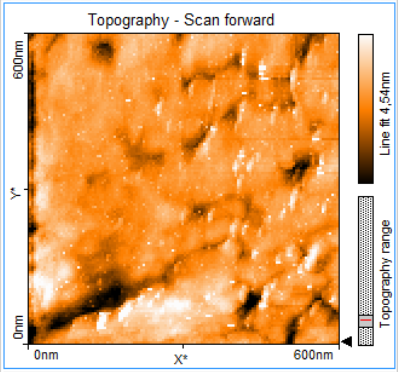
\includegraphics[scale=0.6]{gold_600nm_topographie_oberflaeche.png}
	\caption{Aufnahme der Gold(111)-Schicht mit einer tip-Voltage von 500mV. Im rechten Bereich der Abbildung ist die K�rnige Struktur der Probe gut zu erkennen.}
	\label{fig:gold_maximal_scan}
\end{figure}

In Abbildung \ref{fig:gold_maximal_scan} ist vor allem im rechten Bereich die K�rnige Struktur des Goldes zu sehen. F�r die Aufnahme wurden die Verkippungen bereits korrigiert.

\subsubsection{Rauheit}
F�r die Untersuchung der Oberfl�chen- und Linien Rauheit wurde ein Bereich von 202nm ausgew�hlt. Da ein m�glichst glatter Bereich gew�hlt werden sollte, wurde der obere linke Bereich in aus Abbildung \ref{fig:gold_maximal_scan} ausgew�hlt. In Abbildung \ref{fig:gold_linie} ist eine Aufnahme des Bereichs zu sehen.


\begin{figure}[H]
\centering
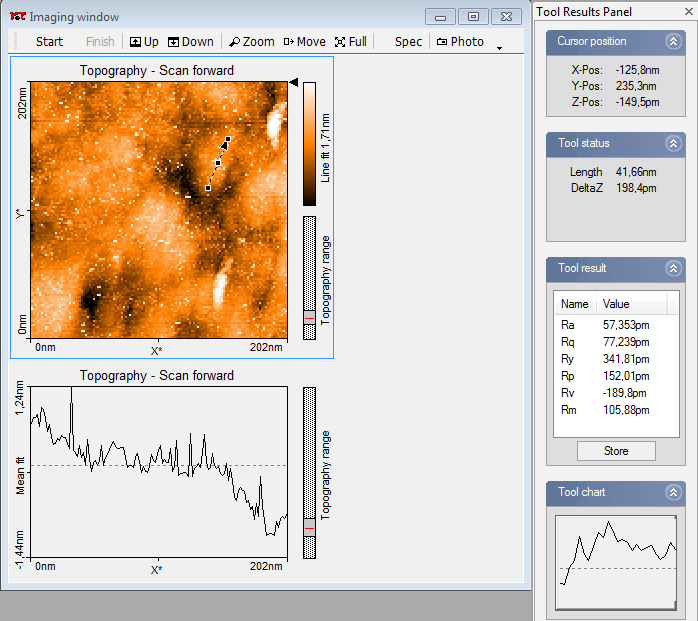
\includegraphics[scale = 0.75]{Gold_linienrauheit_202nm}
\caption{ Mittlere Linienrauheit der (111)-Goldschicht ($R_a = \SI{57,353}{pm}$ und $R_q = \SI{77,239}{pm}$) }
\label{fig:gold_linie}
\end{figure}

\begin{figure}[H]
\begin{subfigure}[t]{0.49\textwidth}
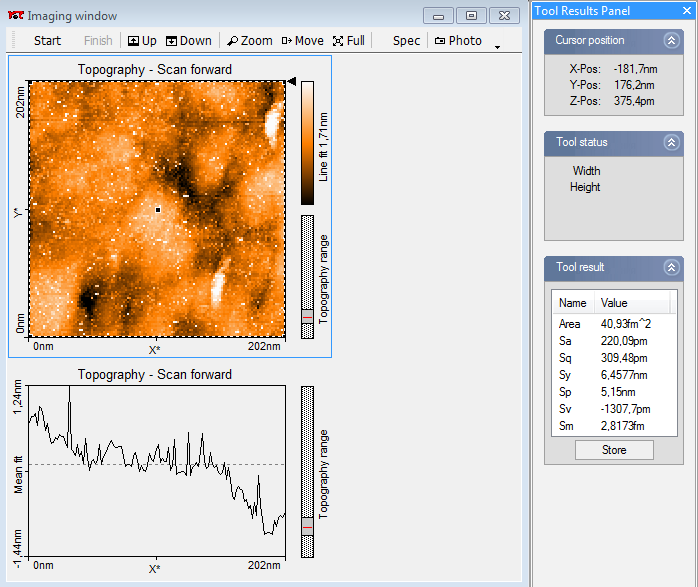
\includegraphics[scale = 0.45]{Gold_flaechenrauheit_202nm_2}
\caption{Mittelung �ber die gesamte Fl�che, da durch die Kornstruktur keine gro�e glatte Fl�che zu finden war. ($S_a = \SI{220,09}{pm}$ und $S_q = \SI{309,48}{pm}$)}
\label{subfig:gold_oberflaeche_1}
\end{subfigure}
\hspace{0.02\textwidth}
\begin{subfigure}[t]{0.49\textwidth}
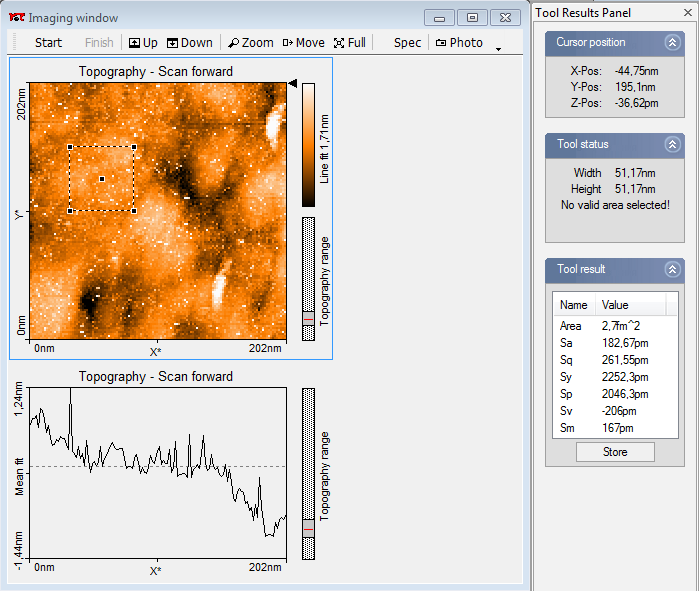
\includegraphics[scale = 0.45]{Gold_flaechenrauheit_202nm_1}
\caption{Mittelung eine kleinere m�glichst glatte Fl�che. Die Verkippung wurde bei allen Messungen korrigiert. ($S_a = \SI{182,67}{pm}$ und $S_q = \SI{261,55}{pm}$)}
\end{subfigure}
\caption{ Mittlere Fl�chenrauheit der (111)-Goldschicht}
\label{subfig:gold_oberflaeche_2}
\end{figure}



Die Oberfl�chenrauheit wird f�r die gesamte Oberfl�che und f�r die glatte Oberfl�che oben links bestimmt (vgl. Abbildung \ref{subfig:gold_oberflaeche_2}). Bei der Bestimmung der Oberfl�chenrauheit, wurden die Werte in Tabelle \ref{tab:rauheit_gold} bestimmt, daf�r wurde die Funktion von easy2Scan verwendet.

\begin{table}[H]
\centering
\caption{Fl�chenrauheit der Goldprobe f�r die gesamter Fl�chen und die Ausschnitt in Abbildung \ref{subfig:gold_oberflaeche_2}}
\label{tab:rauheit_gold}
\begin{tabular}{c|c|c}
Lokalisation & S$_a$ & S$_q$ \\ \hline
\hline Ganzerbereich & 220,09pm & 309,48pm \\ 
\hline Bereich von Abbildung \ref{subfig:gold_oberflaeche_2} & 182,67pm & 261,55pm \\  
\end{tabular} 
\end{table}


Die bestimmten Werte zeigen das an der glatten Stelle die Oberfl�chenrauheit mit S$_a$ 182,67pm um 20\% abweicht. Die Oberfl�chenrauheit auf der gesamten Fl�chen betr�gt S$_a$ = 220,09pm. Die Aufnahme der Linienrauheit ist in Abbildung \ref{fig:gold_linie} zu sehen. Es wurde eine Linienrauheit von R$_a$ = 57,353pm bestimmt, die quadratische Linienrauheit liegt bei R$_q$ = 77,239pm. Die bestimmte Linienrauheit, ist ca. 3 mal so gro� wie die bestimmte Fl�chenrauheit.




\subsubsection{Monoatomare Stufen und Gitterdefekte}

In diesem Abschnitt soll die atomare Struktur der Goldprobe untersucht werden.



